\chapter{Methodology}

\section{Mathematical Concepts Used in the Thesis}\label{section:math_concepts}

This section will provide more specific information about the mathematical concepts used in the implementation part. They are listed below.

\begin{description}
	\item[Equivalent rectangular bandwidth] Equivalent rectangular bandwidth, or ERB, is a measure used for computing bandwidths of the filters for human auditory system. It was defined by Moore and Glasberg in 1983 as \cite{Moore1983}\cite{Holdsworth1988}:
	\begin{equation}
		ERB(f) = 6.23f^2 + 93.39f + 28.52
	\end{equation} 
	
	In 1990, the authors published another approximation (linear) \cite{Moore1990}\cite{Wang2006}:
	\begin{equation}
		ERB(f) = 24.7\,(4.37f + 1)
		\label{equation:ERB_1990}
	\end{equation}
	where $f$ is frequency in kHz.
	
	\item[ERB-rate scale] In psychoacoustics, ERB-rate scale is used to uniformly distribute the filter center frequencies based on their ERB bandwidths. This scale is similar to the critical-band scale of the human auditory system. In 1983, Moore and Glasberg defined it as follows \cite{Moore1983}:
	\begin{equation}
		E(f) = 11.17\ln\left|\frac{f + 0.312}{f + 14.675}\right| + 43.0
	\end{equation}
	
	Using the latest approximation of ERB by Moore and Glasberg (1990), ERB-rate scale function is approximated as \cite{Moore1990}\cite{Wang2006}:
	\begin{equation}
		E(f) = 21.4\log_{10}\left(0.00437f + 1\right)
	\end{equation}
	
	\item[Gammatone filter] A gammatone filter is a linear filter, whose impulse response is a product of a sinusoidal tone and gamma function \cite{Wang2006}:
	\begin{equation}
		g_{f_c}(t) = at^{L-1}\,e^{-2\pi{}tb(f_c)}\,\cos(2\pi{}f_c{}t + \varphi)\,u(t)
		\label{equation:gammatone_impulse_response}
	\end{equation}
	where $a$ is the filter amplitude, $L$ is its order (number of iterations of filtering), $f_c$ is its center frequency, $\varphi$ is the phase, $u(t)$ is the unit-step function ($u(t) = 1$ for $t \ge 0$, and $0$ otherwise), and $b(f_c)$ is the function that determines the bandwidth for a given center frequency \cite{Wang2006}:
	\begin{equation}
		b(f) = 1.019\,ERB(f)
	\end{equation}
	
	Gammatone frequency response is defined as follows \cite{Holdsworth1988}:
	\begin{equation}
		G(f) = \left[1 + \frac{j\,(f - f_c)}{b(f_c)}\right]^{-L} + 
		\left[1 + \frac{j\,(f + f_c)}{b(f_c)}\right]^{-L}
		\qquad\left(-\infty < f < \infty\right)
	\end{equation}
	
	However, when modeling human auditory system, the second term from the definition above can be ignored for sufficiently large $\frac{f_c}{b(f_c)}$ \cite{Wang2006}\cite{Holdsworth1988}:
	\begin{equation}
		G(f)\approx\left[1 + \frac{j\,(f - f_c)}{b(f_c)}\right]^{-L}
		\qquad\left(0 < f < \infty\right)
	\end{equation}
	
	\item[Autocorrelation] Autocorrelation, or autocorrelation function (ACF), is a function that is used to find periodicities and other cues in the input signal. It is defined as the correlation of the signal with its shifted copy. In this thesis the simulated auditory nerve responses will be used to compute it \cite{Wang2006}, and the result will be normalized to receive a set of Pearson's coefficients:
	\begin{equation}
		ACF(n, c, \tau) = \frac{
			\sum\limits_{k=0}^{K-1}a(n - k, c)\,a(n - k -\tau, c)
		}{
			\sqrt{\strut\sum\limits_{\tau}{a^2(n - k, c)}}\,
			\sqrt{\strut\sum\limits_{\tau}{a^2(n - k - \tau, c)}}
		}\,h(k)
	\label{equation:ACF}
	\end{equation}
	where $a(n, c)$ represents the simulated auditory nerve response for frequency channel $c$ and discrete time $n$, $\tau$ is the time lag, $K$ is the length of the sampling window, and $h(k)$ is the window function (usually Hanning, exponential or rectangular).
	
	\item[Summary autocorrelation] Summary autocorrelation function, or SACF, is defined as \cite{Wang2006}\cite{Wang2012}:
	\begin{equation}
		SACF(n, \tau) = \sum_c{ACF(n, c, \tau)}
		\label{equation:SACF}
	\end{equation}
	
	\item[Cross-channel correlation] Cross-channel correlation is a correlation between signals from different frequency channels. In this thesis it is defined for each two neighboring channels ($c$ and $c + 1$) in each time window as normalized correlation \cite{Wang2006}\cite{Wang2012}:
	\begin{equation}
		CCCF(n, c) = \frac{
			\sum\limits_{k=0}^{K-1}a(n - k, c)\,a(n - k, c + 1)
		}{
			\sqrt{\strut\sum\limits_{k=0}^{K-1}{a^2(n - k, c)}}\,
			\sqrt{\strut\sum\limits_{k=0}^{K-1}{a^2(n - k, c + 1)}}
		}h(k)
		\label{equation:CCCF}
	\end{equation}
	where $a(n, c)$ is the simulated auditory nerve response for frequency channel $c$ and discrete time $n$, $K$ is the length of the sampling window, and $h(k)$ is the window function.
\end{description}

\section{Architecture of the System}\label{section:casa_architecture}

Next, to successfully address a concrete implemented system, it is necessary to understand its architecture. The architecture described in the following subsections is based on \cite{Wang2006}, \cite{Wang2012} and \cite{Jasti2020}, though it is impossible to say that it is used in all systems -- in different sources the authors use different approaches and methods, and thus different structures of the models.

\subsection{Peripheral Analysis}\label{subsection:casa_peripheral_analysis}

Usually, a model for computational auditory scene analysis begins with the peripheral analysis of the input sound. Here, first preparations of the input sound for further processing take place. The expected result of this stage includes a time-frequency representation of the input sound -- a set of so-called T-F units. Since the models try to mimic the human cochlea --- and a lot of scientific attention was given to researching it --- the outcome of this stage is almost always a cochleagram.\\

Cochleagrams are in many cases produced by a filterbank of gammatone filters (see chap\-ter~\ref{section:math_concepts} for a definition). Gammatone filters were picked as the most precise ones to simulate points on the basilar membrane of the inner ear. The number of filters in the filterbank might be chosen by the researcher, but the most frequent choice is $128$. The center frequencies of the filters are distributed on the ERB-rate scale (see chapter \ref{section:math_concepts} for a definition), as it was developed to be similar with the critical-band scale of the human auditory system. The filters' impulse and frequency responses are shown on figure \ref{img:gammatone_filterbank}, however it is worth noting that the filters on the figure are normalized, and in practice frequencies higher than 2\,kHz are often amplified \cite{Wang2006}.\\

\begin{figure}[t]
	\centering
	\begin{subfigure}{0.48\textwidth}
		\centering
		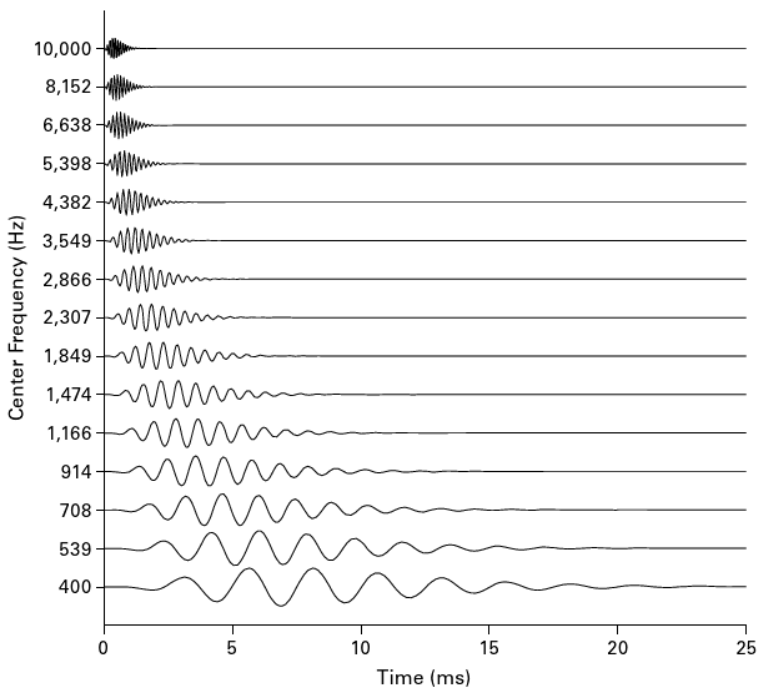
\includegraphics[width=\linewidth]{include/gammatone_filterbank_impulse_response}
		\caption{}
		\label{img:gammatone_filterbank_IR}
	\end{subfigure}%
	\begin{subfigure}{0.52\textwidth}
		\centering
		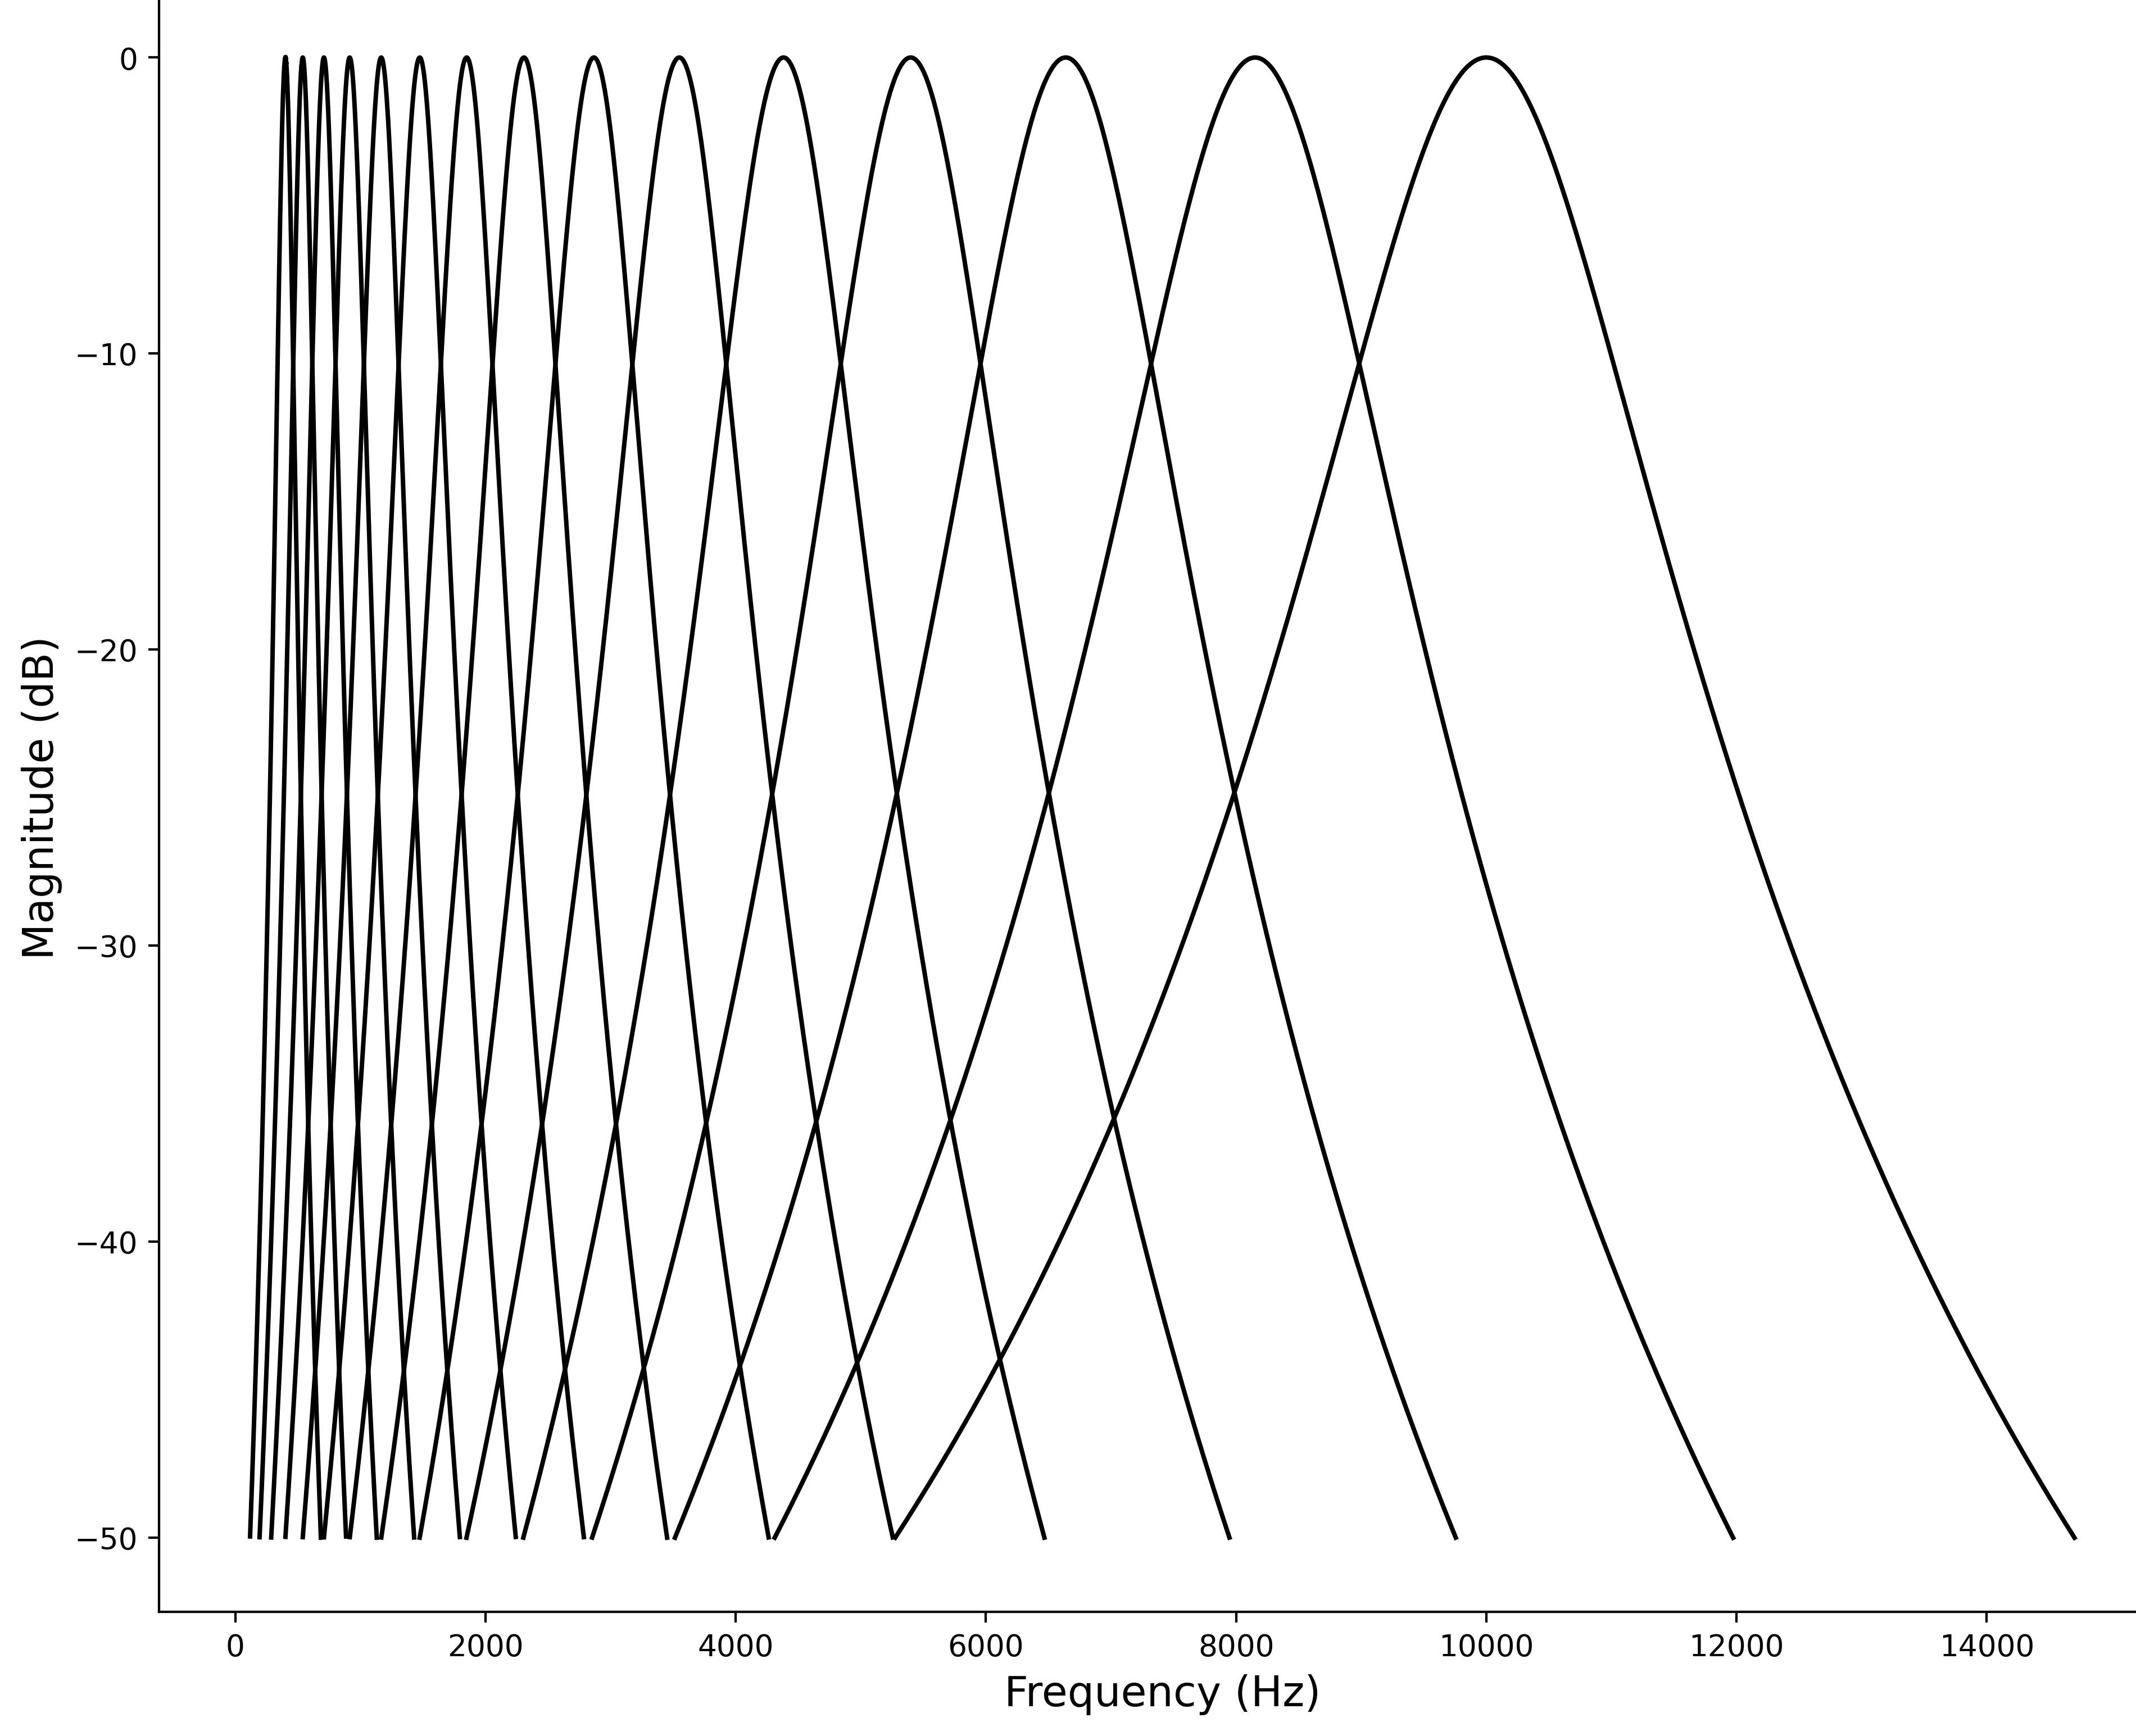
\includegraphics[width=\linewidth]{include/gammatone_filterbank_frequency_response}
		\caption{}
		\label{img:gammatone_filterbank_FR}
	\end{subfigure}
	\caption[Gammatone filterbank impulse and frequency responses]{\textbf{(a)} Impulse responses of $15$ gammatone filters in a gammatone filterbank. The filters' center frequencies are equally spaced between 400\,Hz and 10\,kHz on the ERB-rate scale and are shown on the vertical axis. Taken from \cite{Schnupp2011}. \textbf{(b)} Frequency responses of the same filters. The vertical axis depicts the changes in amplitudes in decibels. Note that the filters with higher center frequencies have wider bandwidths.}
	\label{img:gammatone_filterbank}
\end{figure}

If you look at a cochleagram and a spectrogram of the same sound at the same time, you probably won't notice many differences. The cochleagram similarly shows the densities of frequencies at different points in time, though in this case it may be thought of as a set of frequency channels, where each channel is the output of a certain gammatone filter from the filterbank. The gammatone filters are meant to change the signal so that the frequencies near the center frequency are kept, and the ones that are further away are attenuated (see figure \ref{img:gammatone_filterbank_FR}). At this stage, the windowing techniques described in chapter \ref{section:math_basics} are also used for long signals.

% TODO: Meddis hair cells?

\subsection{Feature Extraction}\label{subsection:casa_feature_extraction}

After the cochleagram is computed, a classic CASA system involves computing a correlogram. In this thesis, correlograms will be put to the feature extraction stage, however some sources discuss them along with the cochleagrams in the peripheral analysis stage \cite{Jasti2020}.\\

According to \cite{Wang2006}, the term correlogram was introduced by Slaney and Lyon in 1990 \cite{Slaney1990} as \textit{"an animated picture of the sound that shows
	frequency content along the vertical axis and time structure along
	the horizontal axis"} (in this thesis the correlogram is a three-dimensional array). The authors used autocorrelation function (see chapter \ref{section:math_concepts} for a definition) on each frequency channel to compute it and described that if the sound is periodic, then the ACF will have peaks in places corresponding to the lags that are equal to the period of repetition. This property of the autocorrelation function has been extensively used in signal processing to estimate pitch and the corresponding fundamental frequencies.\\

So, the fundamental frequency is estimated using the correlogram and the representations of the higher harmonics in it. If you recall the conversation about harmonics from chapter \ref{section:physics_harmonics_pitch}, you may remember that harmonics are periodic at their fundamental frequency, so if the fundamental frequency is, for example, 100\,Hz (the period is 10\,ms), the second harmonic is 200\,Hz (5\,ms), and thus repeats every 10\,ms as well. The correlogram depicts this property in different frequency channels, and when the autocorrelations are summed up, the resulting summary ACF (see chapter \ref{section:math_concepts} for a definition) will have peaks in places corresponding to the period of the fundamental frequency.\\

Of course, correlogram might be used not only for the $f_0$-estimation. In the implementation part, for example, cross-channel correlation is computed from it too. Cross-channel correlation was defined in chapter \ref{section:math_concepts} according to \cite{Wang2012} and may be used to find similarities between units in adjacent frequency channels.\\

Some authors also work with cross-correlograms at this stage. According to \cite{Wang2006}, cross-correlogram is based on the simulated auditory nerve responses from the left and right ears (thus it may be used in binaural systems) and is defined as follows:
\begin{equation}
	CCF(n, c, \tau) = \sum_{k=0}^{K-1} a_L(n-k, c) a_R(n-k-\tau, c) h(k)
\end{equation}
where $a_L(n, c)$ and $a_R(n, c)$ is the above-mentioned simulated auditory nerve response from the left and right ears respectively, $\tau$ is the lag, $h(k)$ is the window function, and $K$ is the size of the sampling window.

\subsection{Mid-Level Representation and Scene Organization}\label{subsection:casa_segmentation_and_grouping}

Next, after the feature extraction stage, follows some work related to segmentation and grouping, which according to Bregman are the main two stages of auditory scene analysis (see chapter \ref{section:biology_asa}). For this part, different authors come up with different names and implementations, but in this thesis it will be split into two stages as in \cite{Wang2006} and \cite{Jasti2020}: mid-level representation and scene organization.\\

Mid-level representation stage includes the first stage of Bregman's ASA --- segmentation. Here, the T-F units computed during the peripheral analysis stage are segregated into segments with the help of the extracted features. These segments, or mid-level representations, are meant to split the cochleagram into separate continuous parts and then are grouped to form auditory streams.\\

Scene organization stage, as it was mentioned, serves to group the mid-level representations into meaningful auditory objects, or streams (see chapter \ref{section:biology_asa}) that come from individual sound sources. Here, for example, separate harmonics are grouped together to form the richer musical sound, or the melody played by the pianist's right hand is grouped with the accompaniment played by the left hand. As a part of this stage, various techniques from the field of artificial intelligence might be used to achieve better results.\\

A notable outcome of this stage is a time-frequency mask of the input cochleagram (or any other chosen T-F representation). The main idea behind masking is to emphasize the T-F units corresponding to the target sound and attenuate those from the background. The mask might have either binary or real values from the $[0, 1]$ interval. If the former method is chosen, the task of searching the T-F mask might be interpreted as a binary classification problem. In case of the latter representation, the values from the mask might be interpreted differently: for example, as the signal-to-noise ratios (SNR) that show the ratios or differences between the target sound energy and overall energy in the T-F unit, or as probabilities that the T-F unit belongs to the target sound \cite{Wang2006}.\\

As it was mentioned earlier, Wang and colleagues \cite{Wang2005} proposed ideal binary mask (IBM) to be the primary goal of CASA. The IBM is defined as follows \cite{Wang2006}\cite{Wang2012}:
\begin{equation}
	IBM(n, c) = 
	\begin{cases}
		1 & \quad\text{if } SNR(n, c) \ge LC \\
		0 & \quad\text{otherwise}
	\end{cases}
\end{equation}
where $SNR(n, c)$ is the signal-to-noise ratio, or the difference between the target sound energy and the interference energy in the T-F unit, and $LC$ is the local criterion chosen as a threshold for the SNR function (most commonly 0\,dB).

\subsection{Resynthesis}\label{subsection:casa_resynthesis}

Finally, some systems include the resynthesis stage to convert the masked T-F representation back to the sound waveform. This is useful for evaluation of the resulting CASA system in cases when listening experiments are held, or signal-to-noise ratios need to be compared before and after the processing \cite{Wang2006}. The technique for resynthesis was proposed by Weintraub in his PhD~thesis in 1985 \cite{Weintraub1985}: the outputs from each gammatone filter in the filterbank were reversed in time to remove the phase shifts, then passed backwards through each filter and reversed back in time again.
